\section{Anchor Analysis on DM, PSD and AMR}
\label{sec:lex:lex-intro}

The 2019 Conference on Computational Language Learning (CoNLL) hosted
a shared task on Cross-Framework Meaning Representation
Parsing~\cite[MRP 2019,][]{Oep:Abe:Haj:19}, which encourage
participants in building a parser for five different meaning
representations in three distinct flavors. \texttt{Flavor-0} includes
the DELPH-IN MRS Bi-lexical Dependencies~\cite[DM,][]{ivanova2012did}
and Prague Semantic
Dependencies~\cite[PSD,][]{hajic2012announcing,miyao2014house}. Both
frameworks under this representation have a syntactic backbone that is
(either natively or by-proxy) based on bi-lexical dependency
structures. As a result, the semantic concepts in these meaning
representations can be anchored to the individual lexical units of the
sentence. \texttt{Flavor-1} includes Elementary Dependency
Structures~\cite[EDS,][]{oepen2006discriminant} and Universal
Conceptual Cognitive Annotation
framework~\cite[UCCA,][]{abend2013universal}, which shows an explicit,
many-to-many anchoring of semantic concepts onto sub-strings of the
underlying sentence. Finally, \texttt{Flavor-2} includes Abstract
Meaning Representation~\cite[AMR,][]{Banarescu:LWPjKI7N}, which is
designed to abstract the meaning representation away from its surface
token. But it leaves open the question of how these are
derived. Previous studies have shown that the nodes in AMR graphs are
predominantly aligned with the surface lexical units, although
explicit anchoring is absent from the AMR representation.  In this
section, we review the related work supporting the claim of the
implicit anchoring in AMR is actually lexical-anchoring, which can be
merged into \texttt{Flavor-0} when we consider the parsing methods on
it.

\subsection{Explicit Alignments: DM, PSD}
\label{ssec:lex:bi-lexical-anchor}
\todo{introduction bi-lexical dependency}


\subsection{Implicit Anchoring in AMR}
\label{ssec:lex:amr-anchor}
AMR tries to abstract the meaning representation away from the surface
token. The absense of explicit anchoring can present difficulties for
parsing. In this section, by extensive analysis on previous work AMR
alignments, we show that AMR nodes can be implicitly aligned to the
leixical tokens in a sentence.

\subsubsection{AMR-to-String Alignments}
\label{sssec:lex:amr2string-align}

A straightforward solution to find the missing anchoring in an AMR Graph is to align it with a
sentence; We denote it as AMR-to-String alignment.

ISI alignments~\cite{Pourdamghani:2014aligning} first linearizes the
AMR graph into a sequence, and then use IBM word alignment
model~\cite{brown1993mathematics} to align the linearized sequence of
concepts and relations with tokens in the sentence. According to the
AMR annotation guidelines and error analysis of ISI aligner, some of
the nodes or relations are evoked by subwords, e.g., the whole graph
fragment \texttt{(p/possible-01 :polarity -)} is evoked by word
``impossible", where the subword \texttt{\char`\"im-\char`\"} actually
evoked the relation polarity and concept \texttt{\char`\"-\char`\"};
On the other side, sometimes concepts are evoked by multiple words,
e.g., named entities, \texttt{(c/city :name (n/name :op1
  \char`\"New\char`" :op2 \char`\"York\char`\"))}, which also happens
in explict anchoring of DM and PSD. Hence, aligning and parsing with
recategorized graph fragments are a natural solution in aligners and
parsers. JAMR aligner~\cite{Flanigan:2014vc} uses a set of rules to
greedily align single tokens, special entities and a set of multiple
word expression to AMR graph fragments, which is widely used in
previous AMR
parsers~\cite[\eg][]{Flanigan:2014vc,Wang:2015uo,Artzi:2009tb,Pust:2015ug,Peng:2015tj,Konstas:2017uj,Wang:2017vt}.

Other AMR-to-String Alignments exists, such as the extended HMM-based
aligner. To consider more structure info in the linearized AMR
concepts, \citet{Wang:2017vt} proposed a Hidden Markov
Model~(HMM)-based alignment method with a novel graph distance. All of
them report over 90\% F-score on their own hand-aligned datasets,
which shows that AMR-to-String alignments are almost token-level
anchoring.

\begin{figure}[t]
\centering
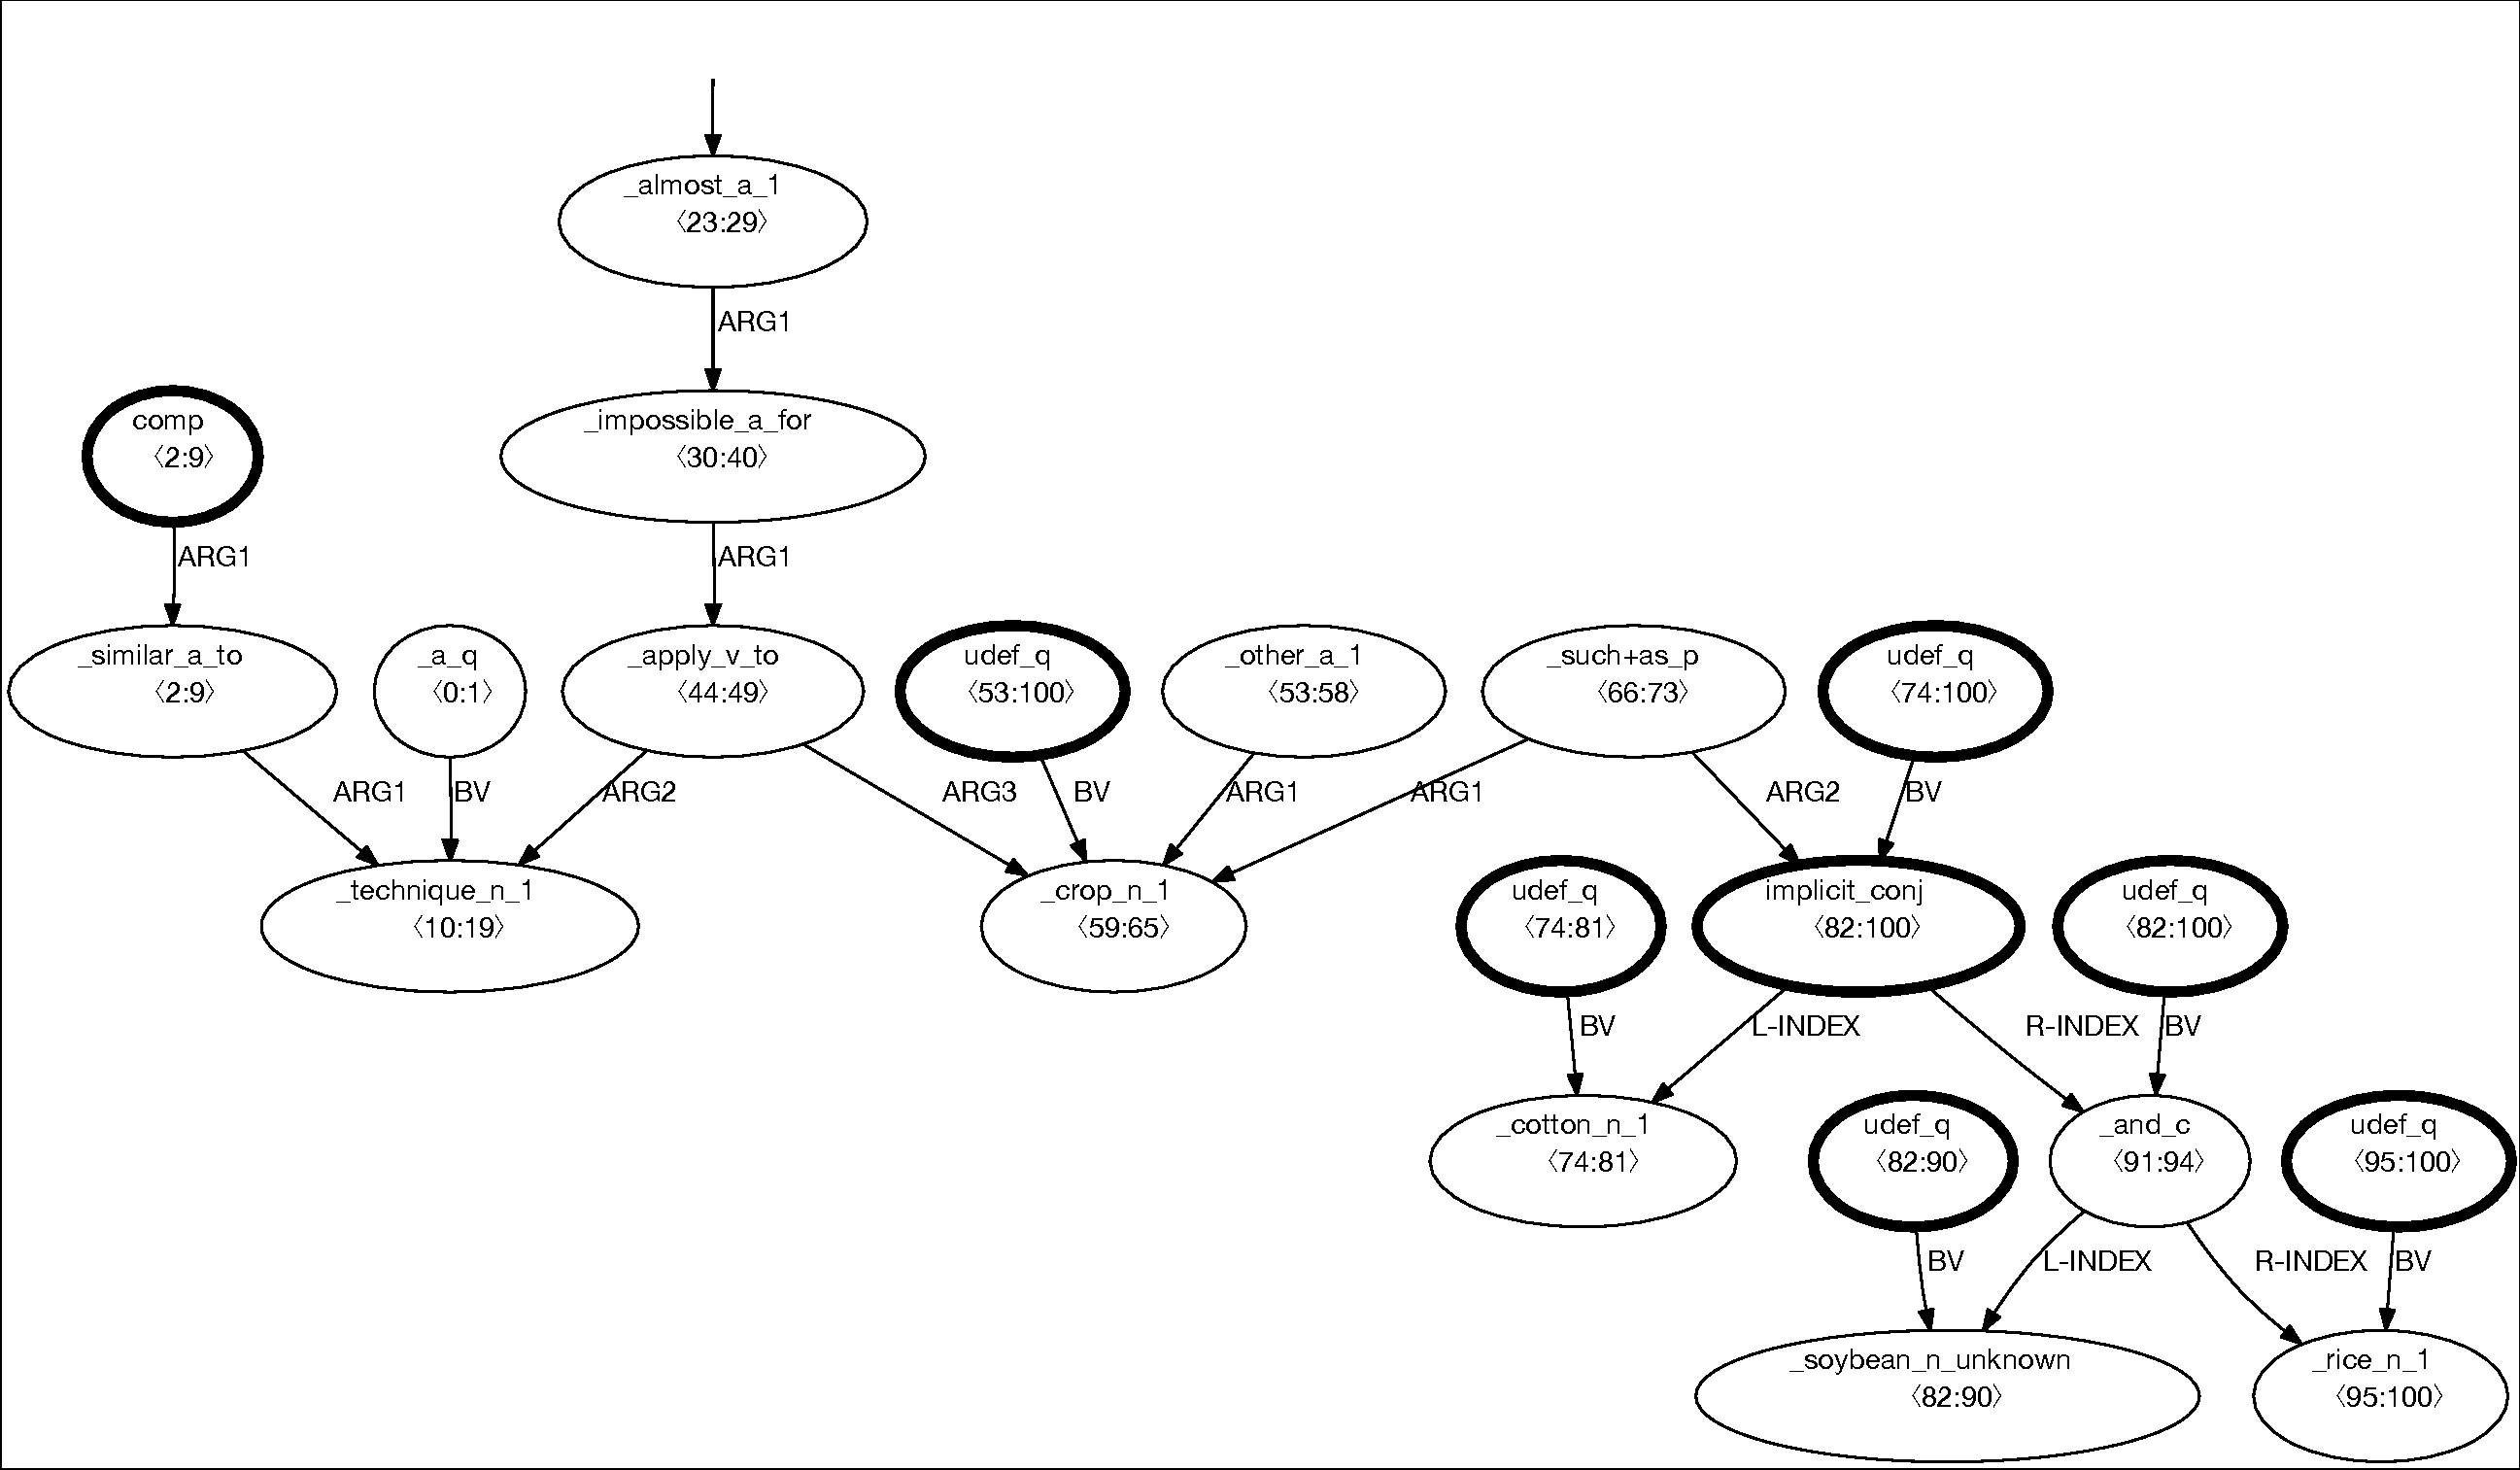
\includegraphics[width=.96\textwidth,trim=.1cm .1cm .05cm .05cm, clip]{eds-white.pdf}
\caption{\label{fig:phrasal-anchoring}Phrasal-anchoring in
  EDS[wsj\#0209013], for the sentence \texttt{\char`\"A similar
    technique is almost impossible to apply to other crops, such as
    cotton, soybeans and rice.\char`\"}. Bold nodes are similar to the
  non-terminal nodes in UCCA, which are anchored multiple tokens, thus
  overlapping with the anchors of other nodes.}
\end{figure}

\subsubsection{AMR-to-Dependency Alignments}
\label{sssec:lex:amr2dep-align}

see \autoref{fig:phrasal-anchoring}
\citet{chen2017unsupervised} first tries to align an AMR graph with a syntactic dependency tree.
\citet{szubert2018structured} conducted further analysis on dependency
tree and AMR interface. It showed 97\% of AMR edges can be evoked by
words or the syntactic dependency edges between words.  Those nodes in
the dependency graph are anchored to each lexical token in the
original sentence. Hence, this observation indirectly shows that AMR
nodes can be aligned to the lexical tokens in the sentence.

Both AMR-to-String and AMR-to-dependency alignments shows that AMR
nodes, including recategorized AMR graph fragements, do have implicit
lexical anchoring. Based on this, \citet{lyu2018amr} propose to treat
token-node alignments as discrete and exclusive alignment matrix and
learn the latent alignment jointly with parsing. Recently,
attention-based seq2graph model also achieved the state-of-the-art
accuracy on AMR parsing~\cite{zhang-etal-2018-stog}.  However, whether
the attention weights can be explained as AMR alignments needs more
investigation in future.

\subsection{Lexical-Anchoring}
\label{ssec:lex:lex-anchor-summary}
According to the bi-lexical dependency structures of DM and PSD, and
implicit lexical token anchoring on AMR, the nodes/categorized graph
fragments of DM, PSD, and AMR are anchored to surface lexical units in
an explicit or implict way. Especially, those lexical units do not
overlap with each other, and most of them are just single tokens,
multiple word expression, or named entities. In other words, when
parsing a sentence into DM, PSD, AMR graphs, tokens in the original
sentence can be merged by looking up a lexicon dict when preprocessing
and then may be considered as a single token for aligning or parsing.

%%% Local Variables:
%%% mode: latex
%%% TeX-master: t
%%% End:
